%
% fig-residuum.tex
%
% (c) 2026 Prof Dr Andreas Müller
%
\begin{figure}
\centering
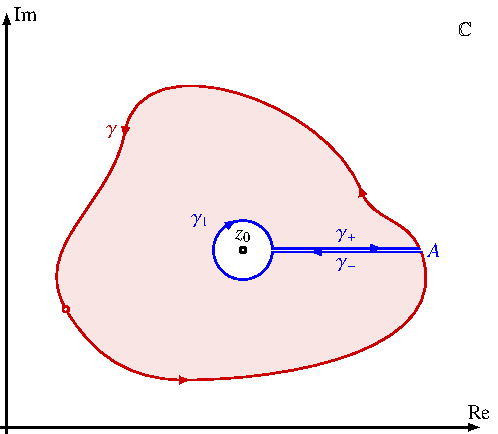
\includegraphics{chapters/030-integration/images/residuum.pdf}
\caption{Herleitung des Integralsatzes.
Der Weg $\gamma$ wird durch die Segmente $\gamma_-$, $\gamma_1$ und
$\gamma_+$ zu einem Weg ergänzt, der das hellrote Gebiet berandet,
in dem die Funktion $f(z)/(z-z_0)$ holomorph ist.
\label{buch:integration:homologie:fig:residuum}}
\end{figure}
